\newpage % Rozdziały zaczynamy od nowej strony.
\cleardoublepage % Zaczynamy od nieparzystej strony
\pagestyle{headings}

\section{Implementacja}

\subsection{Schemat blokowy systemu}

System składa się z dwóch głównych części (Rys. \ref{schemat_blokowy}):
\begin{itemize}
  \item aplikacja wykorzystująca pakiet keras, uruchamiana na komputerze PC
  \item częśc uruchamiana na płytce Z-Turn Board
\end{itemize}

\begin{figure}[h]
  \centering
  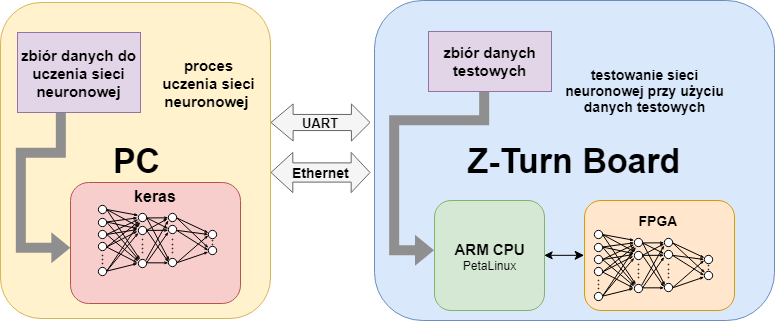
\includegraphics[width=0.8\textwidth]{img/schemat_blokowy.png}
  \caption{Schemat blokowy systemu}
  \label{schemat_blokowy}
\end{figure}


\subsection{Wykorzystanie metody HLS}
Przy użyciu metody HLS możliwe jest stworzenie własnego bloku IP (ang. Intellectual Property), który następnie jest umieszczany w katalogu IP i można go wielokrotnie wykorzystać w projekcie RTL (ang. Register Transfer Level).
Do projektu z użyciem HLS potrzebny jest (Rys.\ref{hls_design_flow}) plik z algorytmem w języku C/C++ lub System C, plik testowy napisany w języku C (ang. testbench) oraz plik z opisem ograniczeń sprzętowych (ang. constraints).
Kolejne etapy projektu z wykorzystaniem metody HLS \cite{hlsXilinxGuide}:

\begin{enumerate}
    \item Kompilacja, wykonanie (symulacja) i debugowanie algorytmu napisanego w języku C
    \item Synteza algorytmu w języku C w implementację RTL
    \item Wygenerowanie raportu i analiza projektu
    \item Zweryfikowanie implementacji RTL
    \item Spakowanie implementacji RTL w blok IP
\end{enumerate}


\begin{figure}
  \centering
  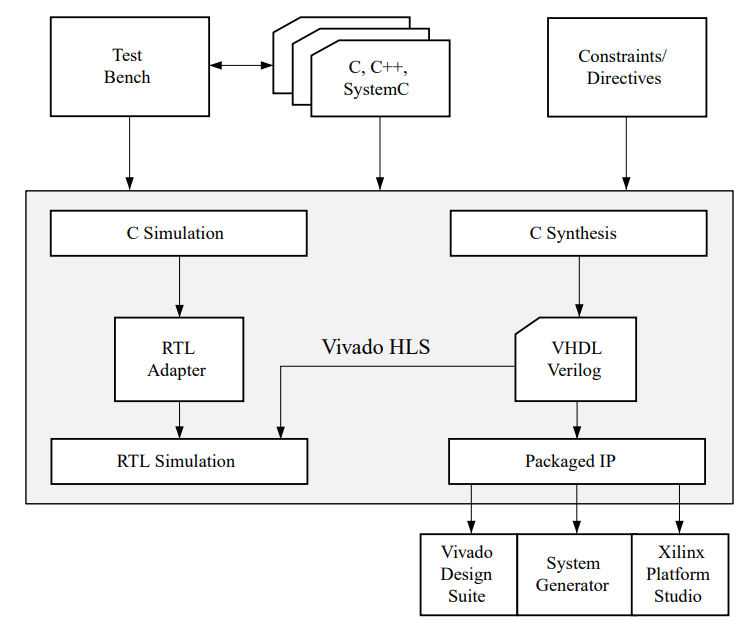
\includegraphics[width=0.8\textwidth]{img/hls_design_flow.png}
  \caption{Proces projektowania przy użyciu metody HLS}
  \label{hls_design_flow}
\end{figure}

Zastosowanie syntezy wysokiego poziomu umożliwia przeniesienie algorytmu napisanego w języku C/C++ lub System C na implementację w układzie FPGA. Dodatkową zaletą metody HLS jest dostępność bibliotek do przetwarzania obrazów oraz ułatwiających implementację operacji matematycznych. 

\subsection{Petalinux}

\subsection{Uczenie Sztucznej Sieci Neuronowej}

\subsection{Zbiór danych wejściowych}

W procesie uczenia oraz testowania poprawności działania modelu sztucznej 
sieci neuronowej wykorzystano zbiór odręcznie pisanych cyfr MNIST 
(ang. THE MNIST DATABASE of handwritten digits)
\cite{lecun-mnisthandwrittendigit-2010}


\subsection{Testowanie systemu}

Algorytmy rozpoznawania obiektów mogą być wywoływane na różne sposoby. 
Jedną z metod jest rejestrowanie obrazu z możliwie maksymalną ilością klatek 
na sekundę, analizowanie każdej ramki, wyszukiwanie obiektów i klasyfikacja za 
pomocą algorytmu ANN. Drugim, prostszym w implementacji sposobem, jest wywoływanie 
zarejestrowania obrazu w momencie, gdy użytkownik, chce dokonać klasyfikacji 
obiektu, który znajduje się w zasięgu obiektywu kamery, a na zarejestrowanym 
obrazie nie ma innych obiektów. Z powodu ograniczeń zasobów systemu, na którym 
aplikacja była testowana oraz ograniczonego czasu wykonania projektu, podjęto 
decyzję o zastosowaniu drugiej metody. 


